%%%% This is based on the Beamer example was created by LianTze Lim, April 2017.

\documentclass[14pt]{beamer}

%%%%%%%%%%%%%%%%%%%%%%%%%%%%%%%%%%%%%%%%%%%%%%%%%%%%%%%%%%%%%%%%%%%%%%%%%%%%%%%%

    \usepackage[catalan]{babel}
    \usepackage[utf8]{inputenc}
    \usepackage[T1]{fontenc}
    \usepackage{lmodern}
    
    \usepackage{xfrac}
    
    %% Set the left and right margins
    \setbeamersize{text margin left=1em,text margin right=1em}

    %% Fonts
    \setbeamerfont{title}{series=\bfseries,size=\huge}
    \setbeamerfont{subtitle}{series=\bfseries,size=\normalsize}
    \setbeamerfont{date}{size=\footnotesize}
    \setbeamerfont{frametitle}{series=\bfseries,size=\normalsize}
    \setbeamerfont{block title}{series=\bfseries,size=\normalsize}
    \setbeamerfont{footline}{size=\normalsize}

    %% Colors
    %\setbeamercolor{background canvas}{bg=white!10!black}   % Blackboard
    %\setbeamercolor{structure}{fg=white!95!black}           % Chalk
    \setbeamercolor{background canvas}{bg=white!99!black}   % background
    \setbeamercolor{structure}{fg=white!05!black}           % foreground
    \usebeamercolor{structure}
    \setbeamercolor{normal text}{fg=structure.fg}

    %% Add a line after the frametitle
    \setbeamertemplate{frametitle}[default][left,leftskip=1ex]
    \addtobeamertemplate{frametitle}{}{\vspace*{-1ex}\rule{\textwidth}{2pt}}

    %% Use circular discs as itemized list markers
    \setbeamertemplate{itemize items}[circle]

    %% Remove default navigation symbols
    \setbeamertemplate{navigation symbols}{}

    %% Remove the footline
    \setbeamertemplate{footline}{}

%%%%%%%%%%%%%%%%%%%%%%%%%%%%%%%%%%%%%%%%%%%%%%%%%%%%%%%%%%%%%%%%%%%%%%%%%%%%%%%%

\title{Parlem de tangrams!}
\subtitle{De la Xina a Egipte passant per Cornellà\ldots}
\author{
    \includegraphics[height=8ex]{figures/figura010a.pdf} \includegraphics[height=8ex]{figures/figura006b.pdf} \includegraphics[height=8ex]{figures/figura010b.pdf} \includegraphics[height=8ex]{figures/figura010c.pdf} 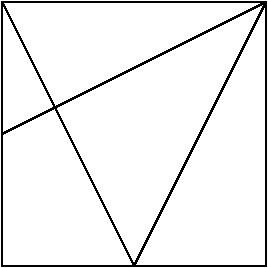
\includegraphics[height=8ex]{figures/figura017.pdf}\\
    \vspace{1.5em}
    \href{https://creativecommons.org/licenses/by-nc-sa/4.0/}{
\includegraphics[scale=0.15]{cc/cc.pdf}
\includegraphics[scale=0.15]{cc/by.pdf}
\includegraphics[scale=0.15]{cc/nc.pdf}
\includegraphics[scale=0.15]{cc/sa.pdf}} \href{https://github.com/CarlosLunaMota}{Carlos Luna-Mota} \\
    29 de gener de 2020 \\
    \vspace{0.75em}
    \href{https://mmaca.cat/}{
\includegraphics[height=3ex]{figures/logo.png}}}
%\date{22 de gener de 2020}

\begin{document}

    \begin{frame}
      \titlepage
    \end{frame}

    %%%%%%%%%%%%%%%%%%%%%%%%%%%%%%%%%%%%%%%%%%%%%%%%%%%%%%%%%%%%%%%%%%%%%%%%%%%%

    \begin{frame}{}
        \begin{center}
            \textbf{\huge Què és un tangram?}\\
        \end{center}
    \end{frame}

    %%%%%%%%%%%%%%%%%%%%%%%%%%%%%%%%%%%%%%%%%%%%%%%%%%%%%%%%%%%%%%%%%%%%%%%%%%%%

    \begin{frame}{Tangram xinès - Dinastia Song (960-1279)}
        \begin{center}
            \includegraphics[height=20ex]{figures/figura001.pdf} \\
        \end{center}
    \end{frame}

    \begin{frame}{Tangram xinès - Siluetes realistes}
        \begin{center}
            \includegraphics[height=15ex]{figures/figura002a.pdf} \quad \phantom{\includegraphics[height=15ex]{figures/figura002b.pdf}} \\
        \end{center}
    \end{frame}

    \begin{frame}{Tangram xinès - Siluetes realistes}
        \begin{center}
            \includegraphics[height=15ex]{figures/figura002a.pdf} \quad \includegraphics[height=15ex]{figures/figura002b.pdf} \\
        \end{center}
    \end{frame}


    \begin{frame}{Tangram xinès - Propietats matemàtiques}
        \begin{center}
            \includegraphics[height=20ex]{figures/figura001.pdf} \\

            \bigskip
            
            \begin{minipage}{0.6\textwidth}
                \begin{description}
                    \item[\textbf{Costats:}] Múltiples d'$1$ i d'$\sqrt{2}$
                    \item[\textbf{Angles:}]  Múltiples de $45^\circ$
                    \item[\textbf{Àrees:}]   Múltiples d'$\sfrac{1}{2}$
                \end{description}
            \end{minipage}
        \end{center}
    \end{frame}

    \begin{frame}{Tangram xinès - Els 13 polígons convexos}
        \begin{center}
            \includegraphics[scale=0.4]{figures/figura003a.pdf}\qquad
            \includegraphics[scale=0.4]{figures/figura003d.pdf}\qquad
            \includegraphics[scale=0.4]{figures/figura003e.pdf}\qquad
            \includegraphics[scale=0.4]{figures/figura003f.pdf}\\ \bigskip
            \begin{tabular}{ccc}
                \includegraphics[scale=0.4]{figures/figura003g.pdf} &
                \includegraphics[scale=0.4]{figures/figura003h.pdf} &
                \includegraphics[scale=0.4]{figures/figura003i.pdf} \\[1ex]
                \includegraphics[scale=0.4]{figures/figura003b.pdf} &
                \includegraphics[scale=0.4]{figures/figura003j.pdf} &
                \includegraphics[scale=0.4]{figures/figura003k.pdf} \\[1ex]
                \includegraphics[scale=0.4]{figures/figura003c.pdf} &
                \includegraphics[scale=0.4]{figures/figura003m.pdf} &
                \includegraphics[scale=0.4]{figures/figura003l.pdf} \\[1ex]
            \end{tabular}\\
        \end{center}
    \end{frame}

    \begin{frame}{Tangram xinès - Paradoxes}
        \begin{center}
            \includegraphics[scale=0.75]{figures/figura004a.pdf}\;\;\qquad\;\phantom{\includegraphics[scale=0.75]{figures/figura004c.pdf}} \\

            \vspace{3em}

            \includegraphics[scale=0.75]{figures/figura004b.pdf}\qquad\phantom{\includegraphics[scale=0.75]{figures/figura004d.pdf}} \\
        \end{center}
    \end{frame}

    \begin{frame}{Tangram xinès - Paradoxes\quad $\mathbf{\left(\sfrac{2\sqrt{2}}{3}\right)^2 = \sfrac{8}{9}}$}
        \begin{center}
            \includegraphics[scale=0.75]{figures/figura004a.pdf}\;\;\qquad\;\includegraphics[scale=0.75]{figures/figura004c.pdf} \\

            \vspace{3em}

            \includegraphics[scale=0.75]{figures/figura004b.pdf}\qquad\includegraphics[scale=0.75]{figures/figura004d.pdf} \\
        \end{center}
    \end{frame}

    \begin{frame}{Altres disseccions}
        \begin{center}
            \includegraphics[scale=0.75]{figures/figura005a.pdf}\qquad\includegraphics[scale=0.75]{figures/figura005b.pdf} \\

            \bigskip

            L'àrea del dodecàgon és $3R^2$
        \end{center}
    \end{frame}

    \begin{frame}{Altres empaquetaments}
        \begin{center}
            \includegraphics[height=12ex]{figures/figura011a.pdf}\qquad\includegraphics[height=12ex]{figures/figura011b.pdf} \\

            \bigskip

            Els dotze pentòminos i els dotze hexamants
        \end{center}
    \end{frame}

    \begin{frame}{Tangrams quadrats}
        \begin{center}
            \includegraphics[height=12ex]{figures/figura006a.pdf}\qquad\includegraphics[height=12ex]{figures/figura006b.pdf}\qquad\includegraphics[height=12ex]{figures/figura006c.pdf}\\

            \bigskip

            Tangram japonès, \emph{Double Square} i tangram Fletcher

            \bigskip

            \includegraphics[height=12ex]{figures/figura030a.pdf}\qquad\includegraphics[height=12ex]{figures/figura030b.pdf}\qquad\includegraphics[height=12ex]{figures/figura030c.pdf}\\

            \bigskip

             Tangram DiDi i altres tangrams de 4 triangles
        \end{center}
    \end{frame}

    \begin{frame}{Tangrams rectangulars}
        \begin{center}
            \includegraphics[height=12ex]{figures/figura007c.pdf}\qquad\quad\includegraphics[height=12ex]{figures/figura007a.pdf}\;\;\phantom{.} \\

            \bigskip
            
            Tangram pitagòric $(4\!\!:\!\!5)$ i tangram \emph{V \& Diamond} $(\sqrt{3}\!\!:\!\!2)$\\

            \bigskip

            \includegraphics[height=12ex]{figures/figura031.pdf}\qquad\includegraphics[height=12ex]{figures/figura007b.pdf}\;\;\phantom{.}\\

            \bigskip
            
            Tangram de la T $(2\!\!:\!\!3)$ i tangram de Brügner $(1\!\!:\!\!\sqrt{\phi})$\\
        \end{center}
    \end{frame}

    \begin{frame}{Tangrams amb corbes}
        \begin{center}
            \includegraphics[height=14ex]{figures/figura008a.pdf}\qquad\qquad\includegraphics[height=14ex]{figures/figura008b.pdf}\\

            \medskip
            
            Tangram de l'ou, tangram del cor i tangrams circulars

            \bigskip

            \includegraphics[height=14ex]{figures/figura008c.pdf}\qquad\qquad\includegraphics[height=14ex]{figures/figura008d.pdf} \\
        \end{center}
    \end{frame}

    %%%%%%%%%%%%%%%%%%%%%%%%%%%%%%%%%%%%%%%%%%%%%%%%%%%%%%%%%%%%%%%%%%%%%%%%%%%%

    \begin{frame}{}
        \begin{center}
            \textbf{\Large Com és un bon tangram?}
        \end{center}
    \end{frame}

    %%%%%%%%%%%%%%%%%%%%%%%%%%%%%%%%%%%%%%%%%%%%%%%%%%%%%%%%%%%%%%%%%%%%%%%%%%%%

    \begin{frame}{Nombre de peces}
        \begin{center}
            \includegraphics[height=15ex]{figures/figura009b.pdf}\qquad\qquad\includegraphics[height=15ex]{figures/figura009a.pdf} \\

            \bigskip
            
            Ostomachion d'Arquimedes i tangram de Brügner
        \end{center}
    \end{frame}

    \begin{frame}{Nombre de peces - Tangrams de 5 peces!}
        \begin{center}
            \includegraphics[height=13ex]{figures/figura010a.pdf}\qquad\includegraphics[height=13ex]{figures/figura010c.pdf}\qquad\includegraphics[height=13ex]{figures/figura010b.pdf} \\

            \bigskip
            
            Subtangram xinès, tangram dels cinc triangles \\
            i tangram de la creu de Sam Loyd
        \end{center}
        \vskip0ptplus1filll\relax
    \end{frame}

    \begin{frame}{Tipus de peces}
        \begin{center}
            \includegraphics[height=13ex]{figures/figura010a.pdf}\qquad\includegraphics[height=13ex]{figures/figura010c.pdf}\qquad\includegraphics[height=13ex]{figures/figura010b.pdf} \\

            \vspace{2em}
            
            \begin{minipage}{0.8\textwidth}
                \begin{itemize}
                    \item Peces senzilles
                    \item Peces diferents
                    \item Peces asimètriques
                    \item Peces d'àrea similar
                \end{itemize}
            \end{minipage}
        \end{center}
        \vskip0ptplus1filll\relax
    \end{frame}

    \begin{frame}{Tipus de peces - Costats i angles compatibles}
        \begin{center}
            \includegraphics[height=13ex]{figures/figura012a.pdf}\qquad\includegraphics[height=13ex]{figures/figura012c.pdf}\qquad\includegraphics[height=13ex]{figures/figura012b.pdf} \\
        \end{center}
        \vskip0ptplus1filll\relax
    \end{frame}

    \begin{frame}{Tipus de peces - Costats i angles compatibles}
        \begin{center}
            \includegraphics[height=13ex]{figures/figura012a.pdf}\qquad\includegraphics[height=13ex]{figures/figura012c.pdf}\qquad\includegraphics[height=13ex]{figures/figura012b.pdf} \\

            \vspace{2em}
            
            \includegraphics[height=13ex]{figures/figura013a.pdf}\qquad\includegraphics[height=13ex]{figures/figura013c.pdf}\qquad\includegraphics[height=13ex]{figures/figura013b.pdf} \\
        \end{center}
        \vskip0ptplus1filll\relax
    \end{frame}


    %%%%%%%%%%%%%%%%%%%%%%%%%%%%%%%%%%%%%%%%%%%%%%%%%%%%%%%%%%%%%%%%%%%%%%%%%%%%

    \begin{frame}{}
        \begin{center}
            \textbf{\huge El tangram egipci}\\

            \bigskip
            
            \textbf{\large un nou tangram \emph{made in} MMACA}
        \end{center}
    \end{frame}

    %%%%%%%%%%%%%%%%%%%%%%%%%%%%%%%%%%%%%%%%%%%%%%%%%%%%%%%%%%%%%%%%%%%%%%%%%%%%
    
    \begin{frame}{Tangram de dues peces}
        \begin{center}
            \includegraphics[height=15ex]{figures/figura014.pdf}\qquad\qquad\phantom{\includegraphics[height=15ex]{figures/figura013b.pdf}} \\

            \vspace{2.5em}

            \includegraphics[height=5ex]{figures/figura015a.pdf}\quad\includegraphics[height=5ex]{figures/figura015b.pdf}\quad\includegraphics[height=5ex]{figures/figura015c.pdf}\;\;\includegraphics[height=5ex]{figures/figura015e.pdf}\quad\includegraphics[height=5ex]{figures/figura015d.pdf}\\
        \end{center}
    \end{frame}

    \begin{frame}{Tangram de dues peces}
        \begin{center}
            \includegraphics[height=15ex]{figures/figura014.pdf}\qquad\qquad\includegraphics[height=15ex]{figures/figura013b.pdf} \\

            \vspace{2.5em}

            \includegraphics[height=5ex]{figures/figura015a.pdf}\quad\includegraphics[height=5ex]{figures/figura015b.pdf}\quad\includegraphics[height=5ex]{figures/figura015c.pdf}\;\;\includegraphics[height=5ex]{figures/figura015e.pdf}\quad\includegraphics[height=5ex]{figures/figura015d.pdf}\\
        \end{center}
    \end{frame}


    \begin{frame}{Tres tangrams de tres peces}
        \vspace{1em}
        \begin{center}
            \includegraphics[height=12ex]{figures/figura016a.pdf}\qquad\includegraphics[height=12ex]{figures/figura016b.pdf}\qquad\includegraphics[height=12ex]{figures/figura016c.pdf} \\
        \end{center}
        \vskip0ptplus1filll\relax
    \end{frame}

    \begin{frame}{Tres tangrams de tres peces}
        \vspace{1em}
        \begin{center}
            \includegraphics[height=12ex]{figures/figura016a.pdf}\qquad\includegraphics[height=12ex]{figures/figura016b.pdf}\qquad\includegraphics[height=12ex]{figures/figura016c.pdf} \\

            \bigskip

            \includegraphics[height=12ex]{figures/figura016d.pdf}\qquad\includegraphics[height=12ex]{figures/figura016e.pdf}\qquad\includegraphics[height=12ex]{figures/figura016f.pdf} \\
        \end{center}
        \vskip0ptplus1filll\relax
    \end{frame}

    \begin{frame}{Tangram egipci}
        \begin{center}
            \includegraphics[height=15ex]{figures/figura017.pdf} \\

            \vspace{2em}

            \begin{minipage}{0.9\textwidth}
                \begin{description}
                    \item[\textbf{Peces:}]   Cinc polígons asimètrics diferents
                    \item[\textbf{Costats:}] Múltiples d'$1$ i d'$\sqrt{5}$
                    \item[\textbf{Angles:}]  Combinacions de $90^\circ$ i de $26,\!565^\circ$
                    \item[\textbf{Àrees:}]   1, 4, 4, 5 i 6
                \end{description}
            \end{minipage}
        \end{center}
    \end{frame}

    \begin{frame}{Tangram egipci - Molts $\mathbf{\left\{1\!\!:\!\!2\!\!:\!\!\sqrt{5}\right\}}$ i un $\mathbf{\left\{3\!\!:\!\!4\!\!:\!\!5\right\}}$}
        \begin{center}
            \includegraphics[height=15ex]{figures/figura018a.pdf}\qquad\includegraphics[height=15ex]{figures/figura018b.pdf} \\

            \bigskip

            Descomposició de les peces del tangram egipci\\ i del tangram de la creu en triangles congruents
        \end{center}
    \end{frame}

    \begin{frame}{Tangram egipci - El quadrilàter és cíclic}
        \vskip0ptplus1filll\relax
        \hspace{4.25em} \includegraphics[scale=1.2]{figures/figura019b.pdf} \\
        \vspace{2.5em}
    \end{frame}

    \begin{frame}{Tangram egipci - Cinc cercles notables}
        \vskip0ptplus1filll\relax
        \hspace{2.66em} \includegraphics[scale=1.2]{figures/figura019.pdf} \\
        \vspace{2.5em}
    \end{frame}

    \begin{frame}{Tangram egipci - Algunes figures}
        \begin{center}
            \raisebox{0ex}{\includegraphics[scale=0.25]{figures/figura022a.pdf}} \quad
            \raisebox{0ex}{\includegraphics[scale=0.25]{figures/figura022b.pdf}} \quad
            \raisebox{0ex}{\includegraphics[scale=0.25]{figures/figura022f.pdf}} \quad
            \raisebox{0ex}{\includegraphics[scale=0.25]{figures/figura022d.pdf}} \quad
            \raisebox{0ex}{\includegraphics[scale=0.25]{figures/figura022c.pdf}} \quad
            \raisebox{0ex}{\includegraphics[scale=0.25]{figures/figura022e.pdf}} \\ \bigskip
            \raisebox{0ex}{\includegraphics[scale=0.25]{figures/figura022l.pdf}} \quad
            \raisebox{0ex}{\includegraphics[scale=0.25]{figures/figura022v.pdf}} \quad
            \raisebox{0ex}{\includegraphics[scale=0.25]{figures/figura022w.pdf}} \quad
            \raisebox{0ex}{\includegraphics[scale=0.25]{figures/figura022x.pdf}} \quad
            \raisebox{0ex}{\includegraphics[scale=0.25]{figures/figura022k.pdf}} \\ \medskip
            \raisebox{0ex}{\includegraphics[scale=0.25]{figures/figura022j.pdf}} \quad
            \raisebox{0ex}{\includegraphics[scale=0.25]{figures/figura022g.pdf}} \quad
            \raisebox{0ex}{\includegraphics[scale=0.25]{figures/figura022h.pdf}} \quad
            \raisebox{0ex}{\includegraphics[scale=0.25]{figures/figura022i.pdf}} \quad
            \raisebox{0ex}{\includegraphics[scale=0.25]{figures/figura022u.pdf}} \\ \bigskip
            \raisebox{1ex}{\includegraphics[scale=0.25]{figures/figura022m.pdf}} \quad
            \raisebox{0ex}{\includegraphics[scale=0.25]{figures/figura022n.pdf}} \quad
            \raisebox{0.4ex}{\includegraphics[scale=0.25]{figures/figura022o.pdf}} \quad
            \raisebox{0.4ex}{\includegraphics[scale=0.25]{figures/figura022r.pdf}} \\
            \raisebox{0ex}{\includegraphics[scale=0.25]{figures/figura022t.pdf}} \quad
            \raisebox{0ex}{\includegraphics[scale=0.25]{figures/figura022s.pdf}} \quad
            \raisebox{-1ex}{\includegraphics[scale=0.25]{figures/figura022p.pdf}} \quad
            \raisebox{0.4ex}{\includegraphics[scale=0.25]{figures/figura022q.pdf}} \\
        \end{center}
    \end{frame}

    \begin{frame}{Tangram egipci - Les tres solucions del quadrat}
        \begin{center}
            \includegraphics[height=12ex]{figures/figura021a.pdf}\quad\includegraphics[height=12ex]{figures/figura021b.pdf}\quad\includegraphics[height=12ex]{figures/figura021c.pdf} \\

            \vspace{2em}

            {\normalsize Quatre angles rectes a l'interior i només dos a la perifèria!}
        \end{center}
    \end{frame}

    \begin{frame}{Tangram egipci - Equivalències i simetries}
        \begin{center}
            \includegraphics[height=8ex]{figures/figura020a.pdf}\quad\includegraphics[height=8ex]{figures/figura020b.pdf}\quad\includegraphics[height=8ex]{figures/figura020c.pdf}\qquad
            \includegraphics[height=8ex]{figures/figura020h.pdf}\quad\includegraphics[height=8ex]{figures/figura020i.pdf} \\ \bigskip
            \includegraphics[height=8ex]{figures/figura020d.pdf}\quad\includegraphics[height=8ex]{figures/figura020f.pdf} \quad \includegraphics[height=8ex]{figures/figura020e.pdf}\quad\includegraphics[height=8ex]{figures/figura020g.pdf} \\ \bigskip
            \includegraphics[height=4ex]{figures/figura020k.pdf}\quad\includegraphics[height=4ex]{figures/figura020j.pdf} \\ \medskip
            \includegraphics[height=4ex]{figures/figura020m.pdf}\quad\includegraphics[height=4ex]{figures/figura020l.pdf} \\
        \end{center}
    \end{frame}

    \begin{frame}{Tangram egipci - Suma de figures semblants}
        \begin{center}
            {\Huge
            \begin{tabular}{ccccc}
                \includegraphics[scale=0.35]{figures/figura025a.pdf} & $=$ &
                \includegraphics[scale=0.35]{figures/figura025b.pdf} & $\!+\!$ &
                \includegraphics[scale=0.35]{figures/figura025c.pdf}\\[1em]
                \includegraphics[scale=0.35]{figures/figura025d.pdf} & $=$ &
                \includegraphics[scale=0.35]{figures/figura025e.pdf} & $\!+\!$ &
                \includegraphics[scale=0.35]{figures/figura025f.pdf}\\
            \end{tabular}}\\
        \end{center}
    \end{frame}

    \begin{frame}{Tangram egipci - Sis triangles semblants}
        \begin{center}
            \includegraphics[scale=0.35]{figures/figura024f.pdf}\quad
            \includegraphics[scale=0.35]{figures/figura024e.pdf}\quad
            \includegraphics[scale=0.35]{figures/figura024d.pdf}\quad
            \includegraphics[scale=0.35]{figures/figura024c.pdf}\quad
            \includegraphics[scale=0.35]{figures/figura024b.pdf}\quad
            \includegraphics[scale=0.35]{figures/figura024a.pdf}\\

            \bigskip

            Triangles semblants d'àrees: 20, 16, 9, 5, 4 i 1
        \end{center}
    \end{frame}
    
    \begin{frame}{Subtangram egipci - Figures amb els 4 triangles}
            \begin{center}
                \begin{tabular}{ccc}
                    \includegraphics[scale=0.35]{figures/figura023a.pdf} &
                    \includegraphics[scale=0.35]{figures/figura023b.pdf} &
                    \includegraphics[scale=0.35]{figures/figura023c.pdf} \\[3ex]
                    \includegraphics[scale=0.35]{figures/figura023d.pdf} &
                    \includegraphics[scale=0.35]{figures/figura023f.pdf} &
                    \includegraphics[scale=0.35]{figures/figura023h.pdf} \\[2ex]
                    \includegraphics[scale=0.35]{figures/figura023e.pdf} &
                    \includegraphics[scale=0.35]{figures/figura023g.pdf} &
                    \includegraphics[scale=0.35]{figures/figura023i.pdf} \\
                \end{tabular}
            \end{center}
    \end{frame}

    %%%%%%%%%%%%%%%%%%%%%%%%%%%%%%%%%%%%%%%%%%%%%%%%%%%%%%%%%%%%%%%%%%%%%%%%%%%%

    \begin{frame}{}
        \begin{center}
            \textbf{\Huge I ara què?}\\
        \end{center}
    \end{frame}

    %%%%%%%%%%%%%%%%%%%%%%%%%%%%%%%%%%%%%%%%%%%%%%%%%%%%%%%%%%%%%%%%%%%%%%%%%%%%

    \begin{frame}{Adaptar el tangram egipci al MMACA}
        \begin{center}
            \includegraphics[height=25ex]{figures/figura027.jpg} \\

            \bigskip
            
            $\mathbf{2+3 = 1+4 = 5}$
        \end{center}
    \end{frame}

    \begin{frame}{Adaptar el tangram egipci a casa i a l'aula}
        \vskip0ptplus1filll\relax

        \vspace{1.75em}
        \begin{itemize}
            \item Paradoxes?
            \item Figures realistes?
            \item Tots els quadrilàters?
            \item Tots els polígons convexos?
            \item Altres activitats didàctiques?
            \item Altres propietats matemàtiques?
            \item \ldots
        \end{itemize}

        %\vspace{0.5em}
        \begin{center}
            {\huge Ajudeu-nos!}\\[1ex]
            \href{mailto:carlos.luna@mmaca.cat}{(carlos.luna@mmaca.cat)}
        \end{center}
    \end{frame}

    \begin{frame}{Antecedents històrics?}
        \vskip0ptplus1filll\relax
        \begin{center}
            \includegraphics[height=15ex]{figures/figura016g.pdf}\qquad\qquad\includegraphics[height=15ex]{figures/figura017b.pdf} \\
        \end{center}
        \vspace{-1em}
        {\footnotesize
        \begin{itemize}
            \item Brunés -- \emph{``The Secrets of Ancient Geometry''} (1967)
            \item Bankoff \& Trigg -- \emph{``The Ubiquitous 3:4:5 Triangle''} (1974)
            \item Detemple \& Harold -- \emph{``A Round-Up of Square Problems''} (1996)
        \end{itemize}}
        \vspace{-1em}
        \begin{center}
            {\huge Ajudeu-nos!}\\[1ex]
            \href{mailto:carlos.luna@mmaca.cat}{(carlos.luna@mmaca.cat)}
        \end{center}
    \end{frame}

    \begin{frame}{Antecedents històrics?}
        \vskip0ptplus1filll\relax
        \begin{center}
            \includegraphics[height=15ex]{figures/figura028a.pdf}\qquad\qquad\includegraphics[height=15ex]{figures/figura028b.pdf} \\

            \bigskip
            
            \hspace{-1em}Puzzle egipci\hspace{6em}\emph{Tangents}\hspace{8em}\\
        \end{center}

        \vspace{0.55em}

        \begin{center}
            {\huge Ajudeu-nos!}\\[1ex]
            \href{mailto:carlos.luna@mmaca.cat}{(carlos.luna@mmaca.cat)}
        \end{center}
    \end{frame}

    \begin{frame}{\hspace{5.25em}{\Large Moltes gràcies!}}
        \vspace{-2em}
        \begin{center}
            \begin{tabular}{ccccc}
                \includegraphics[height=8ex]{figures/figura001.pdf} &
                \includegraphics[height=8ex]{figures/figura010a.pdf} &
                \includegraphics[height=8ex]{figures/figura008a.pdf} &
                \includegraphics[height=8ex]{figures/figura030a.pdf} &
                \includegraphics[height=8ex]{figures/figura007a.pdf} \\           
                \includegraphics[height=8ex]{figures/figura006a.pdf} &
                \includegraphics[height=8ex]{figures/figura010b.pdf} &
                \includegraphics[height=8ex]{figures/figura008b.pdf} &
                \includegraphics[height=8ex]{figures/figura030b.pdf} &
                \includegraphics[height=8ex]{figures/figura007b.pdf} \\           
                \includegraphics[height=8ex]{figures/figura006b.pdf} &
                \includegraphics[height=8ex]{figures/figura010c.pdf} &
                \includegraphics[height=8ex]{figures/figura008c.pdf} &
                \includegraphics[height=8ex]{figures/figura030c.pdf} &
                \includegraphics[height=8ex]{figures/figura007c.pdf} \\           
                \includegraphics[height=8ex]{figures/figura006c.pdf} &
                \includegraphics[height=8ex]{figures/figura017.pdf} &
                \includegraphics[height=8ex]{figures/figura008d.pdf} &
                \includegraphics[height=8ex]{figures/figura009b.pdf} &
                \includegraphics[height=8ex]{figures/figura031.pdf} \\           
            \end{tabular}
        \end{center}
    \end{frame}

\end{document}
